\documentclass[12pt,letterpaper,oneside]{book}
\usepackage[utf8x]{inputenc}
\usepackage[spanish]{babel}
\usepackage{latexsym,amsmath,amssymb,amsthm}
\usepackage{graphicx}
\usepackage{pifont}
\usepackage[pdftex=true,colorlinks=true,plainpages=false]{hyperref}
\hypersetup{urlcolor=blue}
\hypersetup{linkcolor=black}
\hypersetup{citecolor=black}
\usepackage{lastpage}
\usepackage{url}
\usepackage{anysize} 
\marginsize{2.5cm}{1.5cm}{1cm}{1.2cm}
\usepackage{fancyhdr}
\usepackage{tocbibind}

\pagestyle{fancy}
\lhead{\footnotesize \slshape \leftmark} \chead{} \rhead{\footnotesize \slshape \rightmark}
\lfoot{\url{http://scesi.fcyt.umss.edu.bo}}\cfoot{
\includegraphics[scale=0.06]{img/babel.png}}\rfoot{\thepage/\pageref{LastPage}}
\renewcommand{\headrulewidth}{0.4pt}
\renewcommand{\footrulewidth}{0.3pt}
\setlength{\headsep}{0.9\headsep}
\setlength{\footskip}{1.3\footskip}

%\title{Babel}
%\author{Ubaldino Zurita}
%\date{\today}

\begin{document}
 \begin{titlepage}
	\thispagestyle{empty}
	\begin{center}
		
\includegraphics[scale=0.7]{img/babel.png} \\
		~\\
		\Large{\textsc{\bf Universidad Mayor De San Simón}}\\
		\large{\textsc{\bf Facultad De Ciencias y Tecnología}}\\
		\large{\textsc{\bf Sistemas e Informática}}\\
		~\\
		\small{\bf \today}
	\end{center}
 	\vfill
	\begin{center}
		\Huge{\textsc{\bf Manual de Usuario\\ Pagina web BABEL}}
	\end{center}
	\vfill
	\begin{center}

\includegraphics[scale=0.8]{img/licencia.png}
\end{center}
	\hrule
	\vspace{0.1cm}
	\noindent\small{\url{http://scesi.fcyt.umss.edu.bo} \hfill \url{http://www.memi.umss.edu.bo}}
	\hrule
	\vspace{0.1cm}
	\noindent\small{\hspace{1.15cm}
\includegraphics[scale=0.06]{img/scesi2.png} \hfill 
\includegraphics[scale=0.23]{img/memi.jpg}\hspace{0.83cm}}
\end{titlepage}
\thispagestyle{empty}
\begin{center}
%\includegraphics[scale=0.82]{gnome/CreativeCom2.png}\\
%\includegraphics[scale=0.82]{gnome/CreativeCom1.png}  
\end{center}

%\maketitle
\tableofcontents
%\setcounter{page}{1}
\chapter{UTILIZACIÓN DE LA PAGINA}
\section{Interfaz Principal}
Para conectarse a la Pagina web, el Usuario solo necesita ingresar a nuestra pagina web\\ \url{ babel.scesi.memi.umss.edu.bo} Dentro de ella podrá ver un buscador y un menú de catálogos y una opción de acceso para usuarios.
\begin{center}
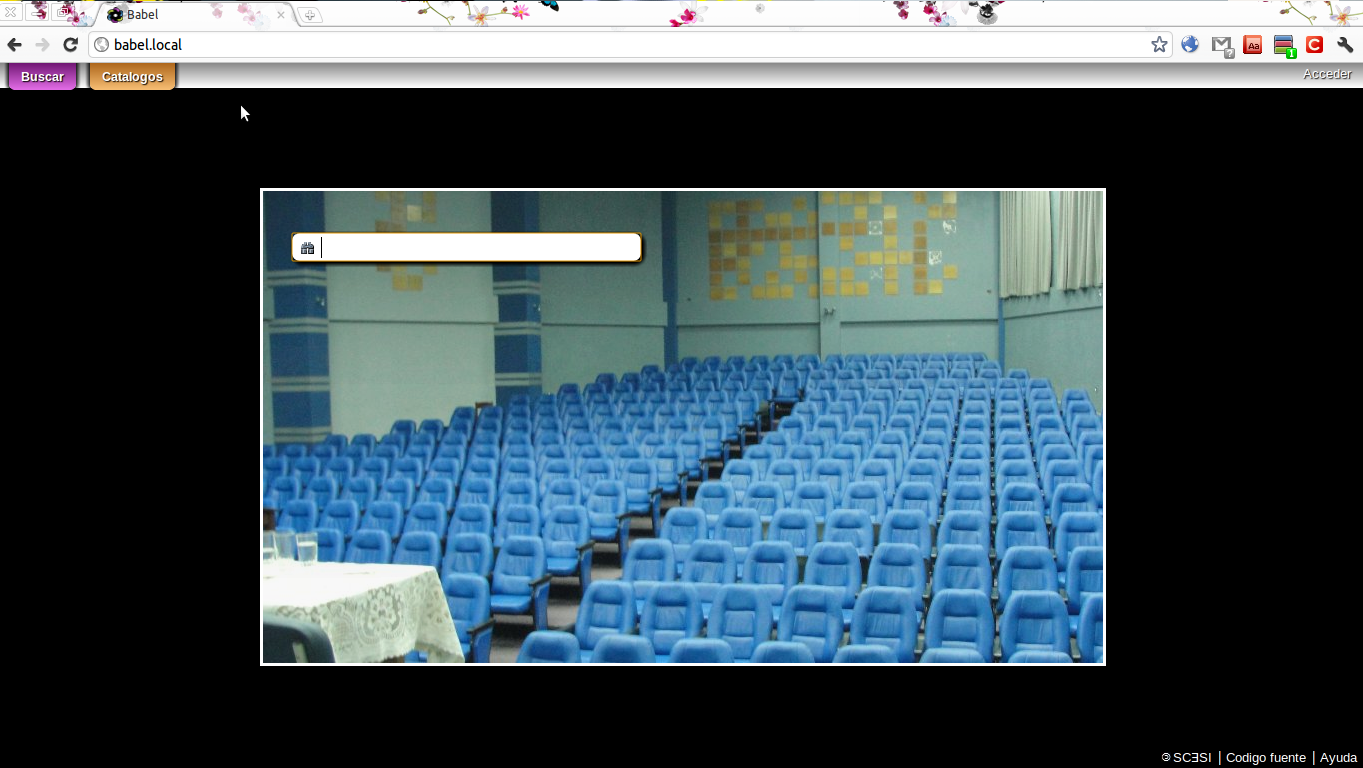
\includegraphics[scale=0.36]{img/1.png}
\end{center}
\section{Búsquedas}
Para la búsqueda de un libro usted solo debe ingresar el nombre del libro que desea y podrá ver resultados asociados a los libros que se encuentran en el sistema.\\
Las búsquedas también tienen una ayuda en la parte inferior derecha.
\begin{center}
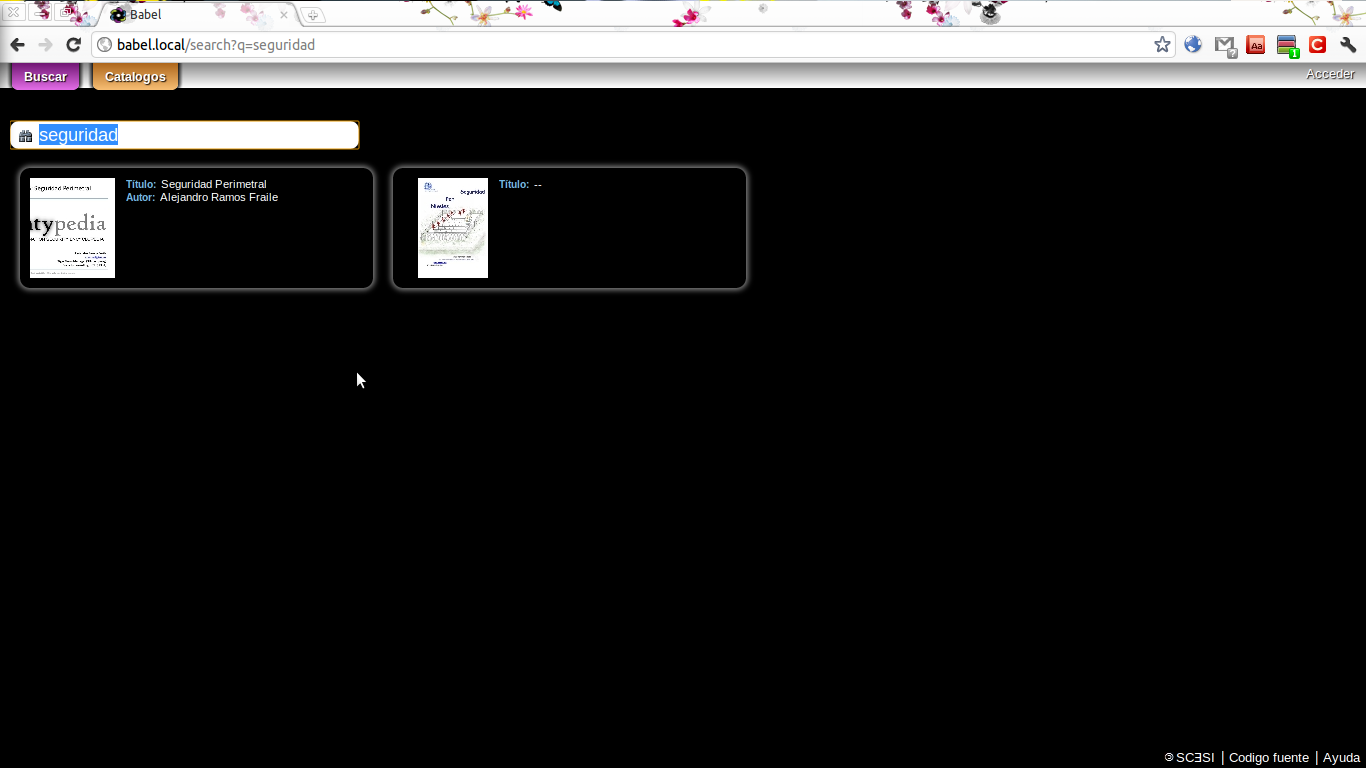
\includegraphics[scale=0.36]{img/2.png}
\end{center}

Para descargar un libro usted solo debe hacer un clic en el icono del diskette y para catalogar el libro debe hacer clic en el siguiente icono.
\begin{center}
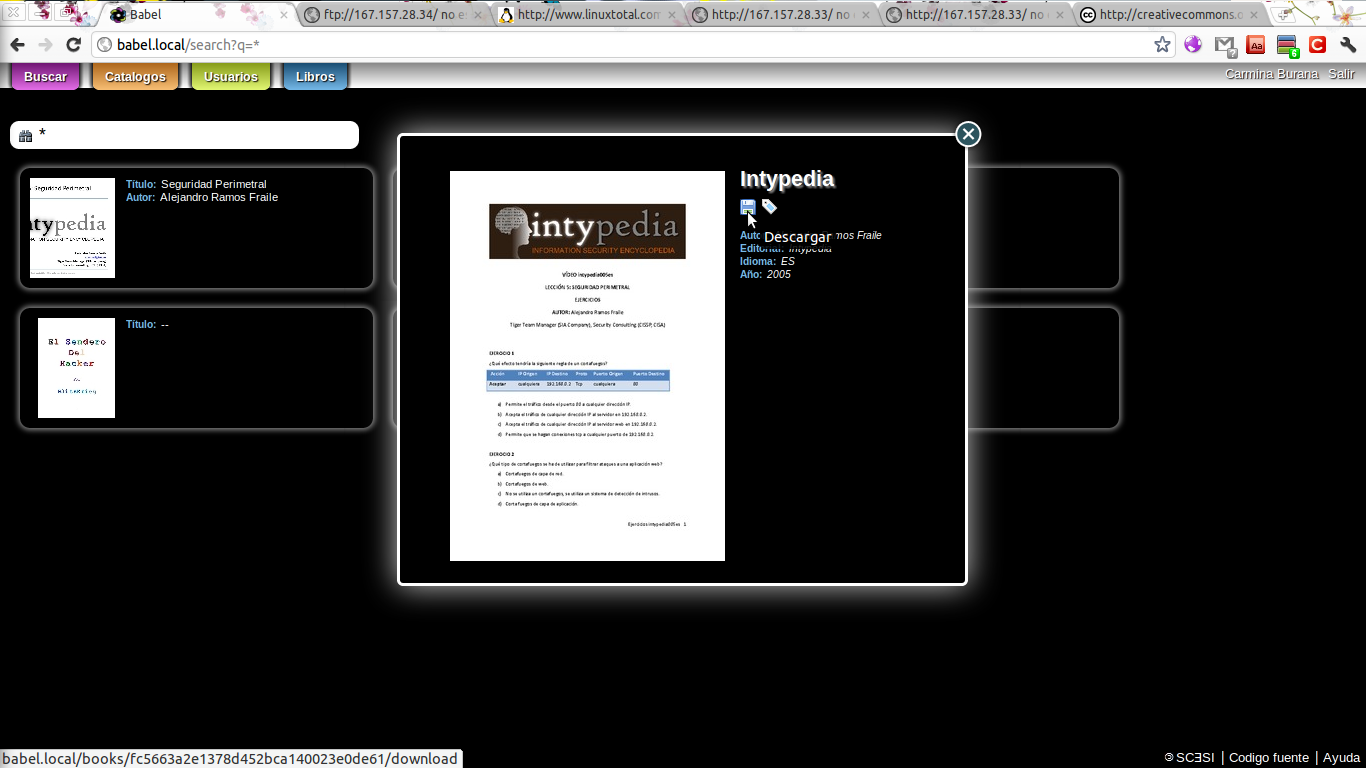
\includegraphics[scale=0.36]{img/3.png}
\end{center}
\pagebreak
\subsection{Búsquedas por Catálogos}
Al hacer clic en el menú Catálogos podrá ver dos opciones:
\begin{itemize}
\item {\bf Lista.}
\item {\bf Nube de Etiquetas.}
\end{itemize}
\begin{description}
\item[Lista.-] Podrá observar catálogos como las Carreras y Generalidades y dentro de cada Catalogo  usted podrá observar Subcatálogos en los que podrá buscar un libro por la Materia o el Área.
\begin{center}
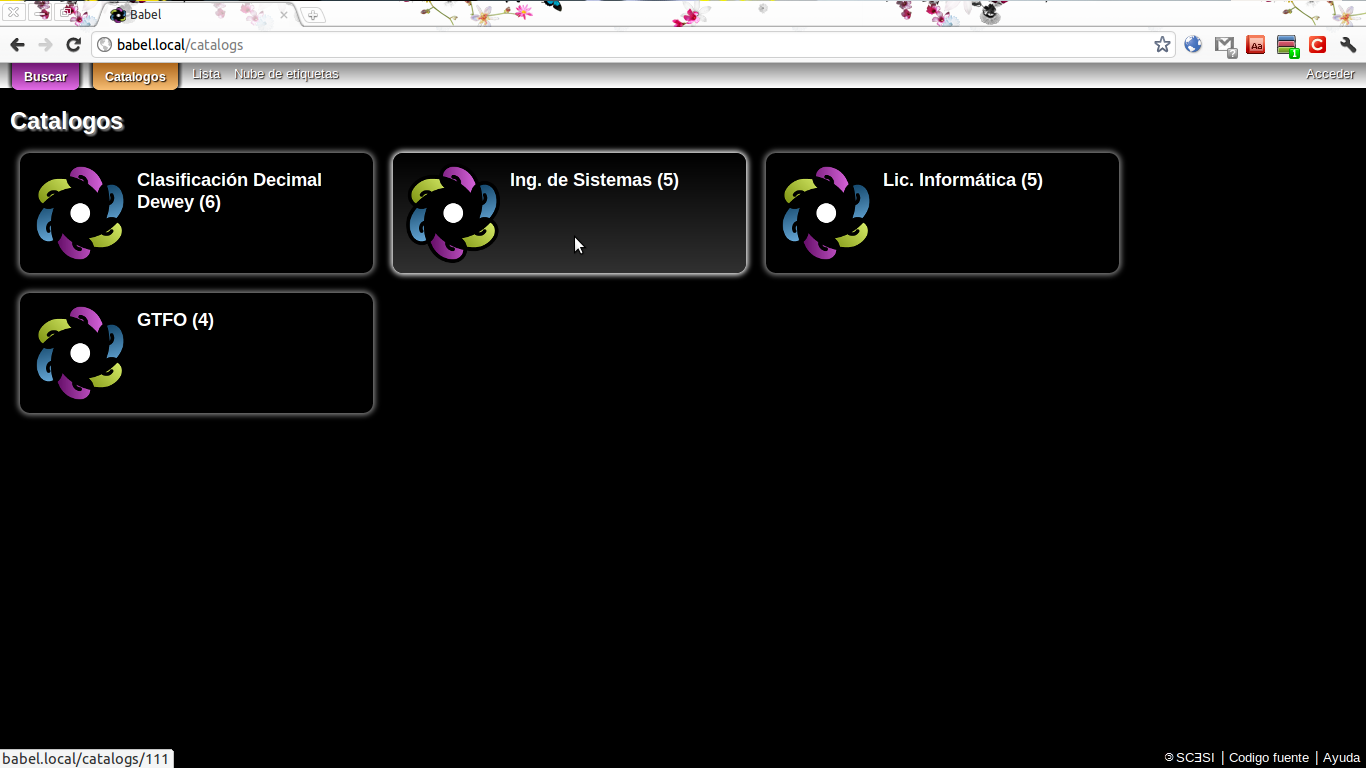
\includegraphics[scale=0.32]{img/4.png}
\end{center}
\item[Nube de etiquetas.-] En esta sección podrá observar las etiquetas realizadas en las materias y carreras
\begin{center}
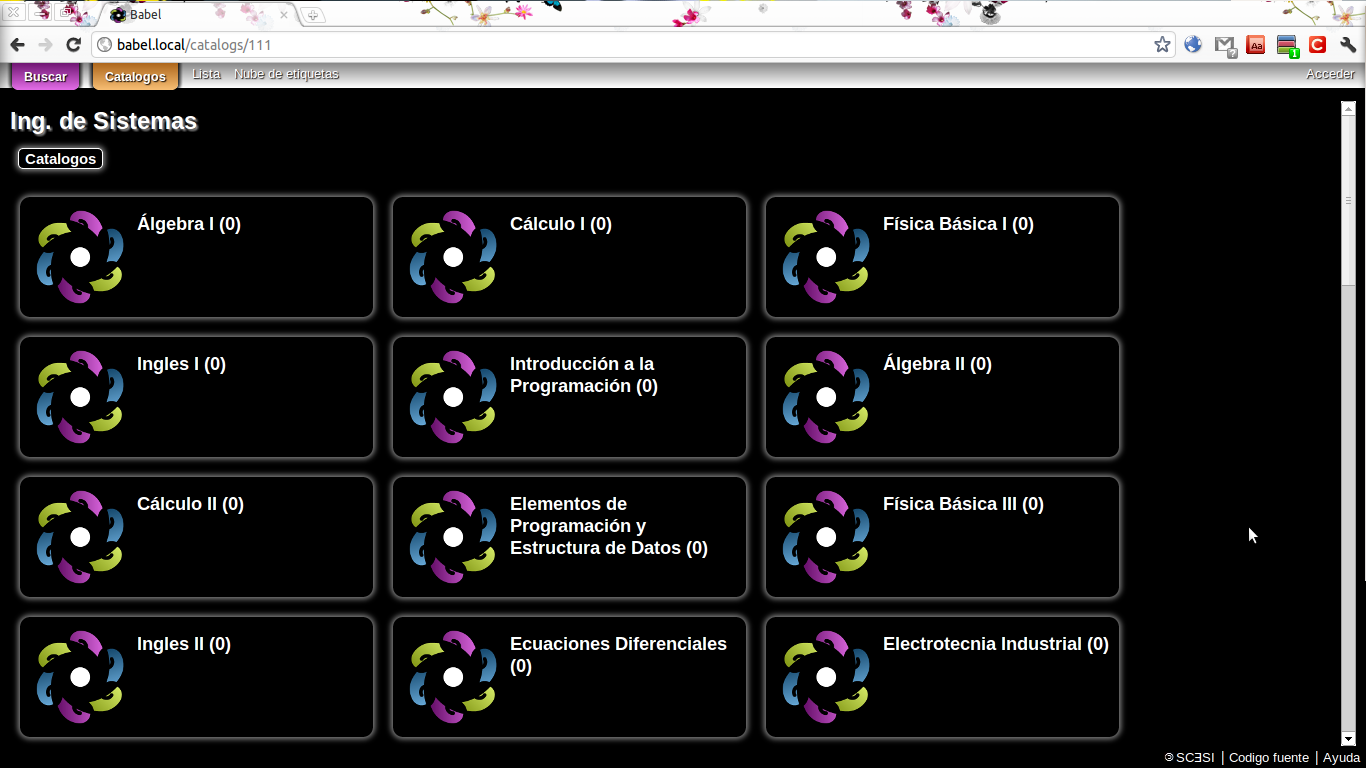
\includegraphics[scale=0.32]{img/5.png}
\end{center}
\end{description}
\section{Obtención de una cuenta de usuario}
Una cuenta de usuario se le asignara a la persona que solicite en inmediaciones de la SCESI.\\
{\bf ¿Como subir un libro?}\\
Para poder subir un libro debe tener una cuenta ftp o puede solicitar en inmediaciones de la SCESI(Sociedad Científica de Estudiante de Sistemas Informática ) que desea publicar un libro. 
%\begin{thebibliography}{5}
%\bibitem{BABEL} BABEL Web-Site: \url{babel.scesi.memi.umss.edu.bo}
%\end{thebibliography}
\end{document}




















